% Gobals
\newcommand{\GetAuthor}{Arne Rick}
\newcommand{\GetTitle}{Implementation of a Planar Strut Network Solver in Python}

% Layout
\documentclass[12pt, oneside]{report}
\usepackage[a4paper,width=150mm,top=25mm,bottom=25mm,bindingoffset=6mm,headheight=15pt]{geometry}
\usepackage[utf8]{inputenc}

\usepackage{parskip}
\usepackage[british]{babel}

\usepackage{graphicx}
\graphicspath{ {images/} }

\usepackage{listings}
\usepackage{solarized-light}
\usepackage{xcolor-solarized}

\lstset{numbers=left,
		numbersep=0.5em,
		numberstyle=\normalfont\footnotesize\color{solarized-violet},
		frame=l,
		framesep=2em,
		framerule=1pt,
		fillcolor=\color{solarized-base2}, 
	    rulecolor=\color{solarized-base2},
	    rulesepcolor=\color{solarized-base2},
	    xleftmargin=2em}

\newenvironment{inconsolata}
	{\fontfamily{fi4}\footnotesize\selectfont}
	{\par}

\usepackage{subfig}
\usepackage{float}
\floatstyle{boxed} 
\restylefloat{figure}

\usepackage{amsmath}
\usepackage{rotating}

\usepackage{tikz}
\usetikzlibrary{calc}

\setcounter{tocdepth}{4}
\setcounter{secnumdepth}{4}

\usepackage{scrextend}

% Notes
\usepackage[colorinlistoftodos,prependcaption,textsize=tiny]{todonotes}
\newcommand{\note}[1]{\todo[linecolor=red,backgroundcolor=red!25,bordercolor=red]{#1}}

% Header and footer
\usepackage{fancyhdr}
\pagestyle{fancy}

\lhead{}
\chead{\GetTitle{}}
\rhead{}

\lfoot{Chapter \thechapter}
\cfoot{\GetAuthor{}}
\rfoot{\thepage}

%\fancyhead{}
%\fancyhead[CO,LE]{\GetTitle{}}
%\fancyfoot{}
%\fancyfoot[LE,RO]{\thepage}
%\fancyfoot[LO,CE]{Chapter \thechapter}
%fancyfoot[CO,RE]{\GetAuthor{}}
\renewcommand{\headrulewidth}{0.4pt}
\renewcommand{\footrulewidth}{0.4pt}

% References
\usepackage{hyperref}
\usepackage[style=numeric]{biblatex}
\addbibresource{references.bib}

\usepackage{cleveref}
\crefname{figure}{figure}{figures}
\Crefname{figure}{Figure}{Figures}

% Title
\title{
	{\GetTitle{}}\\
	{
\includegraphics{hska_logo.png}}
}
\author{\GetAuthor{}}
\date{\today{}, Karlsruhe}

%	Citation
%
%	Education is what remains after one has forgotten what one has learned in school.
%	\parencite[e.g.][page 300]{EIN01}
%

% Document
\begin{document}

% Notes
\newpage
\listoftodos[Notes]
\newpage

\maketitle
\setcounter{page}{1}

\chapter*{Abstract}
Abstract goes here


\chapter*{Acknowledgements}

I would first like to thank my thesis advisor Prof. Marcus Aberle. The door to Prof. Aberle's office was always open whenever I ran into a trouble spot or had a question about my research or writing. He consistently allowed this paper to be my own work, but steered me in the right direction.

I would also like to acknowledge Prof. Dr.-Ing. Markus Baumann as a great mentor and his continuos encouragement in my studies at Hochschule Karlsruhe, University Of Applied Sciences.

I am also grateful to Prof. Dr.-Ing. Robert Pawlowski, lecturer, in the department of Timber Structures, Design and Construction. I am extremly thankful and indebted to him for sharing expertise, and sincere and valuable guidance and encouragement extended to me.

Finally, I must express my very profound gratitude to my parents and to my friends for providing me with unfailing support and continuous encouragement throughout my years of study and through the process of researching and writing this thesis. This accomplishment would not have been possible without them.

And last, but by no means least, I would like thank my friend and roommate Jan Kr\"uger for his support, his insights and for having been there when it mattered most.

Thank you.

\pagestyle{empty}

\tableofcontents

\clearpage
\pagestyle{fancy}

\chapter{Program Structure}
\section{Dependencies}
\label{sec:depend}

Python has a well developed ecosystem of modules and packages to perform advanced tasks.
The modules listed below are used in this implementation.
\bigskip
 
\textit{optparse} [\url{https://docs.python.org/2/library/optparse.html}] \linebreak
The Python option parser \textit{optparse} is used to parse and set defaults for command-line options.
\bigskip

\textit{scipy} [\url{https://www.scipy.org/}]\linebreak
\textit{Scipy} is a widely used Python package for scientific computation. The linear algebra sub-module \textit{linalg} is used in particular to implement the solver (\cref{sec:solver}) routine that solves the system of linear equations describing the system.
\bigskip

\textit{numpy} [\url{https://www.numpy.org/}]\linebreak
\textit{Numpy} is part of the \textit{scipy} package. Apart from the powerful N-dimensional array object used to implement the matrices and vectors several trigonometric functions were used because they are often faster, more stable than the Python math functions and can perform element-wise operations.
\bigskip

\textit{matplotlib} [\url{https://matplotlib.org/}]\linebreak
\textit{Matplotlib} is a powerful Python plotting library. It is used to visualize the system geometry, load vectors, stress resultants and an approximated deflection plot using B\'{e}zier curves.
\bigskip

\textit{csv} [\url{https://docs.python.org/2/library/csv.html}]\linebreak
The \textit{csv} module implements classes to read and write so-called CSV (Comma Separated Values) format spreadsheets used for human readable as well as computer generatable input of system geometry, load vectors, material and profile values, and constraints.
It is also used to store the results (displacement vectors and resultant stresses) of the computation.

\pagebreak

\section{Modules}
\label{sec:modules}

The program is split into multiple modules containing different functions described later in this chapter.

\subsection{main.py}
\label{subsec:main.py}

The main module calls the functions from the different modules and first performs the option parsing.

\begin{inconsolata}
\begin{minipage}{\linewidth}
\begin{lstlisting}[language=python]
...
def main():

    parser = OptionParser(usage="usage: %prog [options]",
                          version="%prog " + str(version))

    # Input Files                                       

    group = OptionGroup(parser, "Input files")

    group.add_option("-N", "--NodeFile",
                     type="string",
                     action="store",
                     dest="nodeFile",
                     default='Input_nodes.csv',
                     help="CSV file with node definitions")
...
\end{lstlisting}
\end{minipage}
\end{inconsolata}

After parsing the command-line options the CSV input files for node, strut, constraint and load definitions are loaded respectively.
Nodes not referenced by any strut (free nodes) are deleted.

\begin{inconsolata}
\begin{minipage}{\linewidth}
\begin{lstlisting}[language=python]
...
    nodes       = readCSV(options.nodeFile,
                          nodesTypeTemplate)

    struts      = readCSV(options.strutFile,
                          strutsTypeTemplate)

    deleteFreeNodes(nodes, struts)

    constraints = readCSV(options.constFile,
                          constraintTypeTemplate)

    strutLoads  = readCSV(options.strutLoadFile,
                          strutLoadTypeTemplate)

    nodeLoads   = readCSV(options.nodeLoadFile,
                          nodeLoadTypeTemplate)
...
\end{lstlisting}
\end{minipage}
\end{inconsolata}

\pagebreak

To validate the references several checks are performed on the data.

\begin{inconsolata}
\begin{minipage}{\linewidth}
\begin{lstlisting}[language=python]
...
    checkStrutNodes(nodes, struts)
    checkConstraintNodes(nodes, constraints)
    checkStrutLoads(struts, strutLoads)
    checkNodeLoads(nodes, nodeLoads)
...
\end{lstlisting}
\end{minipage}
\end{inconsolata}

Properties that can be derived from the inputs (length, angle, type and local member force vector $S\textsubscript{L}$ resulting from the strut loads) and are needed for later computations are calculated and stored in the strut objects.

\begin{inconsolata}
\begin{minipage}{\linewidth}
\begin{lstlisting}[language=python]
...
    getStrutLength(nodes, struts)
    getStrutAngle(nodes, struts)
    getStrutType(struts)
    assemble_S_L(strutLoads, struts, nodes)
...
\end{lstlisting}
\end{minipage}
\end{inconsolata}

The global force vector $S\textsubscript{G}$ is then calculated from node loads and strut loads.

\begin{inconsolata}
\begin{minipage}{\linewidth}
\begin{lstlisting}[language=python]
...
    S_G = assemble_S_G(nodeLoads, struts, nodes)
...
\end{lstlisting}
\end{minipage}
\end{inconsolata}

The system stiffness matrix $K$ is then assembled from the stiffness matrices $K\textsubscript{i}$ of the the individual struts and constraints are applied.

\begin{inconsolata}
\begin{minipage}{\linewidth}
\begin{lstlisting}[language=python]
...
    K = assemble_global_K_I(nodes, struts)
    apply_constraints(K, struts, nodes, constraints)
...
\end{lstlisting}
\end{minipage}
\end{inconsolata}

Now checks can be performed if the system is kinematic. The two criteria used here are:
\begin{itemize}

  \item Under-defined system (not enough constraints)

\begin{equation}
n < 3
\end{equation}

  \item The system stiffness matrix has a non-trivial solution

\begin{equation}
det \lvert K \lvert = 0
\end{equation}

\end{itemize}

\begin{inconsolata}
\begin{minipage}{\linewidth}
\begin{lstlisting}[language=python]
...
    if sp.det(K) == 0:
        print('System is kinematic (det(K)=0)!')
        exit()

    if countConst(constraints) < 3:
        print('System is kinematic (n < 3)!')
        exit()
...
\end{lstlisting}
\end{minipage}
\end{inconsolata}

If these checks are passed the solver can be called to calculate the displacement vector $d$.
After obtaining $d$ the resulting local member forces $S\textsubscript{L}$ can be calculated and stored in the corresponding strut objects.

\begin{inconsolata}
\begin{minipage}{\linewidth}
\begin{lstlisting}[language=python]
...
    d = solver(K, S_G, constraints, nodes)
    calc_local_forces(nodes, struts, d)
...
\end{lstlisting}
\end{minipage}
\end{inconsolata}

Now that the analysis is complete the output can be written to a CSV file and a function called to visualize the system geometry, loads, displacement, deflection and stress resultants.

\begin{inconsolata}
\begin{minipage}{\linewidth}
\begin{lstlisting}[language=python]
...
    writeDisplacements(options.displacementVectorFile,
                       d,
                       nodes)
    drawSystem(nodes,
               struts,
               constraints,
               strutLoads,
               nodeLoads,
               d,
               float(options.scale),
               options.savePlot)
...
\end{lstlisting}
\end{minipage}
\end{inconsolata}


\subsection{util.py}
\label{subsec:util.py}

The utility module contains small helper functions used in all other modules.
These mostly deal with traversing Python's data structures relating names and ids of strut and node objects but also formatting matrices and object properties for debugging output.

\pagebreak

\subsection{input\_templates.py}
\label{subsec:inputtemplates.py}

In order to generate parsers for the CSV input files a template is needed which contains attribute names and type information.

\begin{inconsolata}
\begin{minipage}{\linewidth}
\begin{lstlisting}[language=python]
...
strutsTypeTemplate      = [ ('ID' , str),
                            ('StartNode' , str),
                            ('StartHinge' , int),
                            ('EndNode' , str),
                            ('EndHinge' , int),
                            ('E' , float),
                            ('A' , float),
                            ('I' , float)]
...
\end{lstlisting}
\end{minipage}
\end{inconsolata}

\subsection{input.py}
\label{subsec:input.py}

\textit{input.py} contains the parser generators and type conversion functions used to convert the \textit{string} values from the CSV files to the desired types specified in the corresponding templates.
If conversion fails an error is thrown, telling the user where the malformed input is located.
The functions used to perform checks on the input and derive data used for further computation are also located in this module.

\begin{inconsolata}
\begin{minipage}{\linewidth}
\begin{lstlisting}[language=python]
...
def typeConv(_dict, _typeTemplate):...
def readCSV(csvFile, typeTemplate):...
def genTemplate(filename, typeTemplate):...
def checkStrutNodes(nodes, struts):...
def checkConstraintNodes(nodes, constraints):...
def checkStrutLoads(struts, strutLoads):...
def checkNodeLoads(nodes, nodeLoads):...
def deleteFreeNodes(nodes, struts):...
def getStrutLength(nodes, struts):...
def getStrutAngle(nodes, struts):...
def getStrutType(struts):...
def strutLength(strut, nodes):...
def strutAngle(strut, nodes):...
def strutType(strut):...
\end{lstlisting}
\end{minipage}
\end{inconsolata}

\subsection{output.py}
\label{subsec:output.py}

The functions of the \textit{output} module are used to convert and store the results of the analysis in CSV files.

\pagebreak

\subsection{solver.py}
\label{subsec:solver.py}

The \textit{solver} module implements the routine to solve the system of linear equations using methods form the \href{http://www.netlib.org/lapack/}{LAPACK} package contained in \textit{scipy}:

\begin{equation}
S\textsubscript{G} = K \cdot d
\end{equation}

After computing the solution the constraints are applied to the resulting vector $d$.

\begin{inconsolata}
\begin{minipage}{\linewidth}
\begin{lstlisting}[language=python]
...
def solver(K, S_G, constraints, nodes):
    d = sp.solve(K,S_G)

    #apply constraints: set d[i] = 0
    for ID, const in constraints.iteritems():
        id = nodeNameToID(const['Node'], nodes)
        if const['x']:
            x = id * 3
            d[x] = 0
        if const['z']:
            x = id * 3 + 1
            d[x] = 0
        if const['r']:
            x = id * 3 + 2
            d[x] = 0

    return d
\end{lstlisting}
\end{minipage}
\end{inconsolata}

\pagebreak

\subsection{load\_vectors.py}
\label{subsec:loadvectors.py}

This module encompasses all function definitions to calculate the local member forces $S\textsubscript{L}$ \cite[4.2-4.11]{schneider} resulting from the different load vectors (\cref{fig:loadVec}) for each member type (\cref{fig:memberTypes}).


\begin{figure}[h]%
    \centering
    \subfloat[Type 1: trapazoid]{{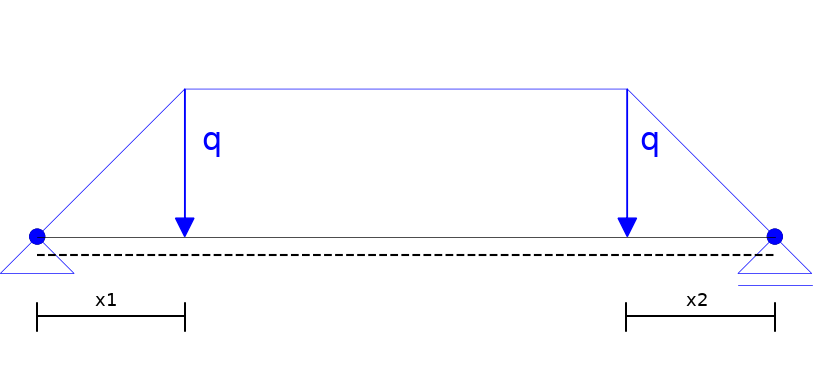
\includegraphics[width=0.4\textwidth]{load_type_1.png}}}%
    \qquad
    \subfloat[Type 2: torque]{{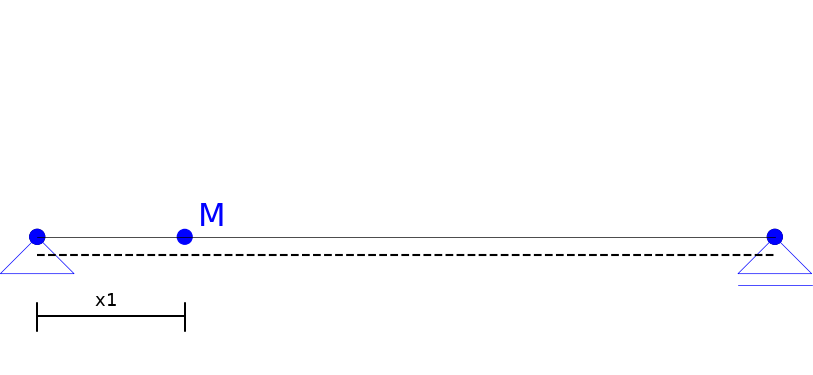
\includegraphics[width=0.4\textwidth]{load_type_2.png}}}%

    \centering
    \subfloat[Type 3: force]{{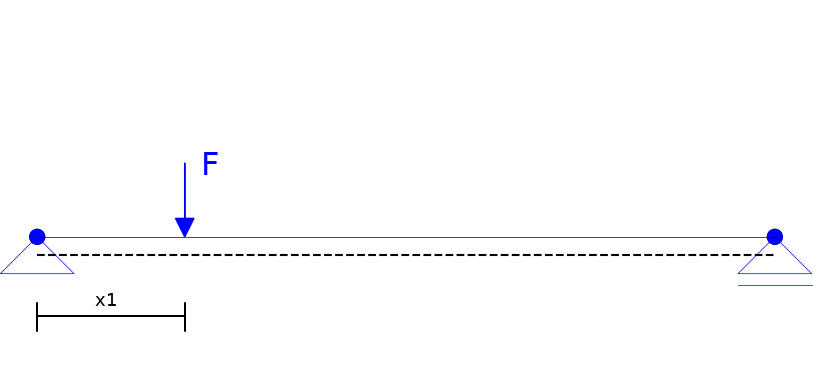
\includegraphics[width=0.4\textwidth]{load_type_3.png}}}%
    
    \caption{Load Vectors}%
    \label{fig:loadVec}%
\end{figure}


\begin{figure}[h]%
    \centering
    \subfloat[Type 1: both joints rigid]{{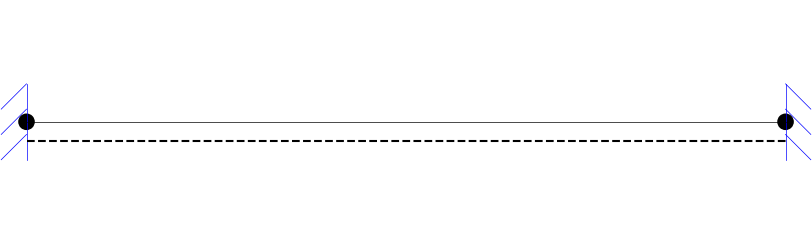
\includegraphics[width=0.4\textwidth]{strut_type_1.png}}}%
    \qquad
    \subfloat[Type 2a: right: pin-jointed, left: rigid joint]{{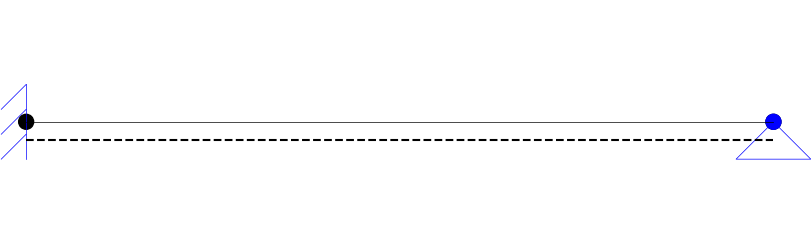
\includegraphics[width=0.4\textwidth]{strut_type_2a.png}}}%

    \centering
    \subfloat[Type 2b: right: rigid joint, left: pin-jointed]{{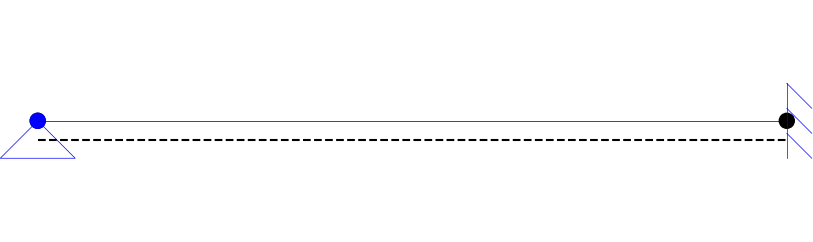
\includegraphics[width=0.4\textwidth]{strut_type_2b.png}}}%
    \qquad
    \subfloat[Type 3: both pin-jointed]{{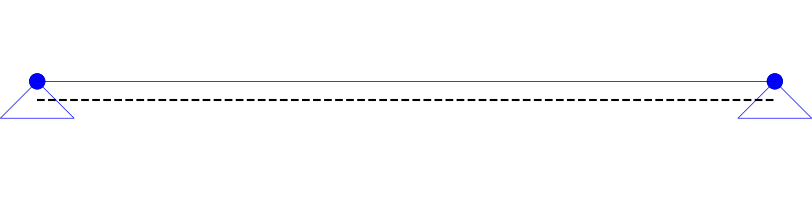
\includegraphics[width=0.4\textwidth]{strut_type_3.png}}}%
    
    \caption{Member Types}%
    \label{fig:memberTypes}%
\end{figure}

\begin{inconsolata}
\begin{minipage}{\linewidth}
\begin{lstlisting}[language=python]
...
def S_L_1_1( x1, x2, l, F, M, q ):...
def S_L_1_2a( x1, x2, l, F, M, q ):...
def S_L_1_2b( x1, x2, l, F, M, q ):...
def S_L_1_3( x1, x2, l, F, M, q ):...

def S_L_2_1( x1, x2, l, F, M, q ):...
def S_L_2_2a( x1, x2, l, F, M, q ):...
def S_L_2_2b( x1, x2, l, F, M, q ):...
def S_L_2_3( x1, x2, l, F, M, q ):...

def S_L_3_1( x1, x2, l, F, M, q ):...
def S_L_3_2a( x1, x2, l, F, M, q ):...
def S_L_3_2b( x1, x2, l, F, M, q ):...
def S_L_3_3( x1, x2, l, F, M, q ):...
...
\end{lstlisting}
\end{minipage}
\end{inconsolata}

The function references are stored in a \textit{dictionary} and dereferenced by member and load type as keys to simplify the implementation of the \textit{get\_S\_L} function and allow for easy expandability.

\begin{inconsolata}
\begin{minipage}{\linewidth}
\begin{lstlisting}[language=python]
...
dict = {
    1:{
        '1'  : S_L_1_1,
        '2a' : S_L_1_2a,
        '2b' : S_L_1_2b,
        '3'  : S_L_1_3
    },
    2:{
        '1'  : S_L_2_1,
        '2a' : S_L_2_2a,
        '2b' : S_L_2_2b,
        '3'  : S_L_2_3
    },
    3:{
        '1'  : S_L_3_1,
        '2a' : S_L_3_2a,
        '2b' : S_L_3_2b,
        '3'  : S_L_3_3
    }
}

#calculates the load vector from a load
def get_S_L( load, strut):
    x1 = load['x1']
    x2 = load['x2']
    l  = strut['l']
    F  = load['F']
    M  = load['M']
    q  = load['q']
    loadType = load['Type']
    strutType = strut['Type']

    return dict[loadType][strutType](x1, x2, l, F, M, q)
...
\end{lstlisting}
\end{minipage}
\end{inconsolata}

A function to assemble the global load vector $S\textsubscript{G}$ from the local member forces $S\textsubscript{L}$ by rotating them to global coordinates ($S\textsubscript{G} = S\textsubscript{L} \cdot rot(\alpha)$ (\cref{rot})) and the node loads by simply adding them to the vector is also part of the module.

\begin{equation} \label{rot}
rot = \begin{pmatrix}
cos(\alpha)  & sin(\alpha)  & 0   & 0             & 0             & 0   \\[0.2em]
-sin(\alpha) & cos(\alpha)  & 0   & 0             & 0             & 0   \\[0.2em]
0            & 0            & 1   & 0             & 0             & 0   \\[0.2em]
0            & 0            & 0   & cos(\alpha)   & sin(\alpha)   & 0   \\[0.2em]
0            & 0            & 0   & -sin(\alpha)  & cos(\alpha)   & 0   \\[0.2em]
0            & 0            & 0   & 0             & 0             & 1
     \end{pmatrix}
\end{equation}

\begin{inconsolata}
\begin{minipage}{\linewidth}
\begin{lstlisting}[language=python]
...
#creates the global load vector from strut loads and node loads
def assemble_S_G( nodeLoads, struts, nodes ):
    size = len(nodes) * 3
    S_G = np.zeros(size)

    #add node loads
    for ID, load in nodeLoads.iteritems():
        id = nodeNameToID(load['Node'], nodes)
        Fx = load['Fx']
        Fz = load['Fz']
        M  = load['M']
        v = np.array([Fx, Fz, M])
        for i in range(3):
            S_G[id*3 + i] += v[i]

    #add strut load vectors
    for ID, strut in struts.iteritems():
        id = nodeNameToID(strut['StartNode'], nodes)

        S_L = np.zeros(6)
        if 'S_L' in strut:
            S_L = strut['S_L']

        #rotate to global coordinates
        alpha = strut['alpha']
        v = rot(alpha).dot(S_L)
        for i in range(6):
            S_G[id*3 + i] += v[i] * -1

    return S_G
...
\end{lstlisting}
\end{minipage}
\end{inconsolata}

\subsection{matrices.py}
\label{subsec:matrices.py}

\textit{matrices} is used to deal with the required matrix operations and to calculate the matrices of the different member types (\cref{fig:memberTypes}).
\note{reference matrices}
\begin{equation} \label{K1}
K\textsubscript{1} = \begin{pmatrix}
\dfrac{EA}{l} & 0                   & 0                   & -\dfrac{EA}{l}  & 0                   & 0                   \\[0.8em]
              & 2d\dfrac{EI}{l^3}   & -d\dfrac{EI}{l^2}   & 0               & -2d\dfrac{EI}{l^3}  & -d\dfrac{EI}{l^2}   \\[0.8em]
              &                     & a\dfrac{EI}{l}      & 0               & d\dfrac{EI}{l^2}    & b\dfrac{EI}{l}      \\[0.8em]
              &                     &                     & 0               & \dfrac{EA}{l}       & 0                   \\[0.8em]
              &                     &                     &                 & 0                   & d\dfrac{EI}{l^2}    \\[0.8em]
              &                     &                     &                 &                     & a\dfrac{EI}{l}
     \end{pmatrix}
\end{equation}

\begin{equation} \label{K2a}
K\textsubscript{2a} = \begin{pmatrix}
\dfrac{EA}{l} & 0                   & 0                   & -\dfrac{EA}{l}  & 0                   & 0                   \\[0.8em]
              & c\dfrac{EI}{l}      & -c\dfrac{EI}{l^2}   & 0               & -\dfrac{EI}{l^3}    & 0                   \\[0.8em]
              &                     & c\dfrac{EI}{l}      & 0               & c\dfrac{EI}{l^2}    & 0                   \\[0.8em]
              &                     &                     & \dfrac{EA}{l}   & 0                   & 0                   \\[0.8em]
              &                     &                     &                 & c\dfrac{EI}{l^3}    & 0                   \\[0.8em]
              &                     &                     &                 &                     & 0
     \end{pmatrix}
\end{equation}

\begin{equation} \label{K2b}
K\textsubscript{2b} = \begin{pmatrix}
\dfrac{EA}{l} & 0                   & 0                   & -\dfrac{EA}{l}  & 0                   & 0                   \\[0.8em]
              & \dfrac{EI}{l^3}     & 0                   & 0               & -c\dfrac{EI}{l^3}   & -c\dfrac{EI}{l^2}   \\[0.8em]
              &                     & 0                   & 0               & 0                   & 0                   \\[0.8em]
              &                     &                     & \dfrac{EA}{l}   & 0                   & 0                   \\[0.8em]
              &                     &                     &                 & c\dfrac{EI}{l^3}    & c\dfrac{EI}{l^2}    \\[0.8em]
              &                     &                     &                 &                     & c\dfrac{EI}{l}
     \end{pmatrix}
\end{equation}

\begin{equation} \label{K3}
K\textsubscript{3} = \begin{pmatrix}
\dfrac{EA}{l} & 0                   & 0                   & -\dfrac{EA}{l}  & 0                   & 0                   \\[0.8em]
              & 0                   & 0                   & 0               & 0                   & 0                   \\[0.8em]
              &                     & 0                   & 0               & 0                   & 0                   \\[0.8em]
              &                     &                     & \dfrac{EA}{l}   & 0                   & 0                   \\[0.8em]
              &                     &                     &                 & 0                   & 0                   \\[0.8em]
              &                     &                     &                 &                     & 0
     \end{pmatrix}
\end{equation}

The member coeffecient $\varepsilon$ is dependent on the strut length $l$, the normal force $N$ and its flexural rigidity $EI$:

\begin{equation} \label{e}
\varepsilon = l \cdot \sqrt{\frac{|N|}{EI}}
\end{equation}

The coefficients $a, b, c ,d$ are functions in second order theory and model stiffening and weakening due to normal force.
In first order theory ($N = 0 \Rightarrow \varepsilon = 0$) they are treated as constants.
\note{reference coefficients}
\begin{equation} \label{a}
    a = \begin{cases}
            \hfil 4              & \text{if } \varepsilon \leq 0\\[1.2em]
            \hfil \dfrac{\varepsilon \cdot sin(\varepsilon) - \varepsilon^2 \cdot cos(\varepsilon)}{2 \cdot (1 - cos(\varepsilon)) - (\varepsilon \cdot sin(\varepsilon))}               & \text{if } N < 0          \\[1.2em]
            \dfrac{\varepsilon \cdot sinh(\varepsilon) - \varepsilon^2 \cdot cosh(\varepsilon)}{2 \cdot (cosh(\varepsilon) - 1) - \varepsilon \cdot sinh(\varepsilon)}               & \text{if } N > 0
        \end{cases}
\end{equation}

\begin{equation} \label{b}
    b = \begin{cases}
            \hfil 2              & \text{if } \varepsilon \leq 0\\[1.2em]
            \hfil \dfrac{\varepsilon^2 - \varepsilon \cdot sin(\varepsilon)}{2\cdot(1 - cos(\varepsilon)) - \varepsilon \cdot sin(\varepsilon) }               & \text{if } N < 0          \\[1.2em]
            \dfrac{\varepsilon^2 - \varepsilon \cdot sinh(\varepsilon))}{2 \cdot (cosh(\varepsilon) - 1) - \varepsilon \cdot sinh(\varepsilon)}               & \text{if } N > 0
        \end{cases}
\end{equation}

\begin{equation} \label{c}
    c = \begin{cases}
            \hfil 3              & \text{if } \varepsilon \leq 0\\[1.2em]
            \hfil \dfrac{\varepsilon^2 \cdot sin(\varepsilon)}{sin(\varepsilon) - \varepsilon \cdot cos(\varepsilon)}               & \text{if } N < 0          \\[1.2em]
            \dfrac{\varepsilon^2 \cdot sinh(\varepsilon)}{\varepsilon \cdot cosh(\varepsilon) - \varepsilon \cdot sinh(\varepsilon)}               & \text{if } N > 0
        \end{cases}
\end{equation}

\begin{equation} \label{d}
    d = a + b
\end{equation}

Because all matrices are symmetric the lower left is left empty (initiated with $0$). All matrix operations are only applied to the upper right parts to save time.
Only the \textit{solver} (\cref{subsec:solver.py}) requires that the entries are mirrored to the lower left. Therefore, when the system stiffness matrix $K$ is assembled it gets symmetrized before calling the \textit{solver} by adding the transposed matrix to itself and subtracting the diagonal.
This assumes that the lower left contains only zeroes.

\begin{equation} \label{symmetrize}
    M\textsubscript{sym} = M + M^\top - diag(M)
\end{equation}


\begin{inconsolata}
\begin{minipage}{\linewidth}
\begin{lstlisting}[language=python]
...
def symmetrize(M):
    return M + M.T - np.diag(M.diagonal())
...
\end{lstlisting}
\end{minipage}
\end{inconsolata}

\begin{figure}[h!]%
    \centering
    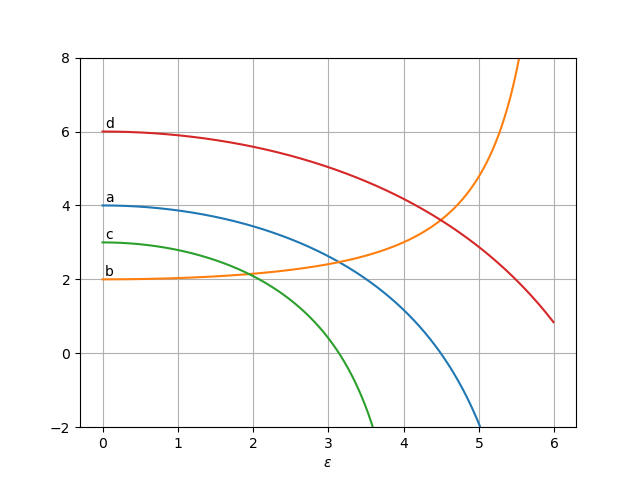
\includegraphics[width=0.9\textwidth]{coeff_N_neg.png}%
    \caption{Coefficients for negative normal pressure}%
    \label{fig:coeff_N_neg}%
\end{figure}

\begin{figure}[h!]%
    \centering
    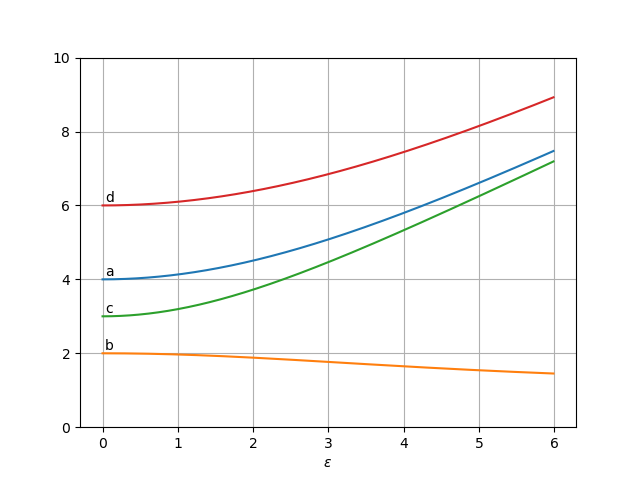
\includegraphics[width=0.9\textwidth]{coeff_N_pos.png}%
    \caption{Coefficients for positive normal pressure}%
    \label{fig:coeff_N_pos}%
\end{figure}

\pagebreak

\subsection{graphics.py}
\label{subsec:graphics.py}

The \textit{graphics} module is used to visualize the system geometry, load vectors, stress resultants and to generate an approximated deflection plot.
The plots can be displayed directly and execution is blocked or saved to a .png or .pdf file.

\note{Update when drawSystem shows resultants}
\begin{inconsolata}
\begin{minipage}{\linewidth}
\begin{lstlisting}[language=python]
...
def drawSystem(nodes, struts, constraints,
               strutLoads, nodeLoads,
               d,
               size,
               savePlot):
    
    _min, _max, mid = getBounds(nodes)
    fig, ax = plt.subplots() 

    # Nodes
    drawNodes(nodes, size, ax)

    # Constraints
    drawConstraints(constraints, nodes, mid, size, ax)

    # Struts
    drawStruts(struts, nodes, size, ax)
    
    ##########################################################

    # Displaced nodes
    drawDisplacedNodes(d, nodes, size, ax)

    # Displaced struts
    drawDisplacedStruts(struts, nodes, size, ax)

    ##########################################################

    # loads
    drawStrutLoads(strutLoads, size, struts, nodes, ax)
    drawNodeLoads(nodeLoads, size, struts, nodes, ax)

    ###########################################################

    # Extend plot for margin
...
    
    # Label
    plt.title("System")
    
    # Same scale on both axes
    ax.set_aspect('equal')

    if savePlot != False:
        # saves plot in file
        plt.savefig(savePlot, bbox_inches='tight')
    else:
        # shows the plot
        plt.show()
...
\end{lstlisting}
\end{minipage}
\end{inconsolata}

\pagebreak



\chapter{IO}
\section{Option Parsing}
\label{sec:optparse}

Option parsing is implemented using \textit{Pyhtons} \textit{optparse} (\cref{sec:depend}). The options are split into four groups:

\begin{itemize}
\item Input Files

-N NODEFILE, --NodeFile=NODEFILE

\textit{CSV file with node definitions}

-S STRUTFILE, --StrutFile=STRUTFILE

\textit{CSV file with strut definitions}

-C CONSTFILE, --ConstraintFile=CONSTFILE

\textit{CSV file with constraint definitions}

-L STRUTLOADFILE, --StrutLoadFile=STRUTLOADFILE

\textit{CSV file with strut load definitions}

-F NODELOADFILE, --NodeLoadFile=NODELOADFILE

\textit{CSV file with node load definitions}

-T 

\textit{Generate csv input template files}

\item Output Files

-D DISPLACEMENTVECTORFILE,\\
--DisplacementVectorFile=DISPLACEMENTVECTORFILE 

\textit{Destination path to save the displacement vector csv file}

\item Graphics

-s SCALE, --Scale=SCALE

\textit{Scales plot elements}

-P SAVEPLOT, --SavePlot=SAVEPLOT

\textit{Destination path to save the system plot. Supported filetypes: .png, .pdf}

\item Debug
-d, --Debug

\textit{Print debug outputs}
\end{itemize}

\begin{inconsolata}
\begin{minipage}{\linewidth}
\begin{lstlisting}[language=python]
...
    parser = OptionParser(usage="usage: %prog [options]",
                          version="%prog " + str(version))

################################################################
#       Input files                                            #
################################################################

    group = OptionGroup(parser, "Input files")

    group.add_option("-N", "--NodeFile",
                     type="string",
                     action="store",
                     dest="nodeFile",
                     default='Input_nodes.csv',
                     help="CSV file with node definitions")

    group.add_option("-S", "--StrutFile",
                     type="string",
                     action="store",
                     dest="strutFile",
                     default='Input_struts.csv',
                     help="CSV file with strut definitions")

    group.add_option("-C", "--ConstraintFile",
                     type="string",
                     action="store",
                     dest="constFile",
                     default='Input_constraints.csv',
                     help="CSV file with constraint definitions")

    group.add_option("-L", "--StrutLoadFile",
                     type="string",
                     action="store",
                     dest="strutLoadFile",
                     default='Input_strutLoads.csv',
                     help="CSV file with strut load definitions")

    group.add_option("-F", "--NodeLoadFile",
                     type="string",
                     action="store",
                     dest="nodeLoadFile",
                     default='Input_nodeLoads.csv',
                     help="CSV file with node load definitions")

    group.add_option("-T",
                     action="store_true",
                     dest="genTemplates",
                     help="Generate csv input template files")

    parser.add_option_group(group)
...
\end{lstlisting}
\end{minipage}
\end{inconsolata}

\begin{inconsolata}
\begin{minipage}{\linewidth}
\begin{lstlisting}[language=python]
...
################################################################
#       Output files                                           #
################################################################

    group = OptionGroup(parser, "Output files")

    group.add_option("-D", "--DisplacementVectorFile",
                     type="string",
                     action="store",
                     dest="displacementVectorFile",
                     default='displacement.csv',
                     help="Destination path to save the displacement vector csv file")

    parser.add_option_group(group)
...
\end{lstlisting}
\end{minipage}
\end{inconsolata}

\begin{inconsolata}
\begin{minipage}{\linewidth}
\begin{lstlisting}[language=python]
...
################################################################
#       graphics                                               #
################################################################

    group = OptionGroup(parser, "Graphics options")

    group.add_option("-s", "--Scale",
                     type="float",
                     action="store",
                     dest="scale",
                     default=2.0,
                     help="Scales plot elements")

    group.add_option("-P", "--SavePlot",
                     type="string",
                     action="store",
                     dest="savePlot",
                     default=False,
                     help="Destination path to save the system plot. Supported filetypes: .png, .pdf")

    parser.add_option_group(group)
...
\end{lstlisting}
\end{minipage}
\end{inconsolata}

\begin{inconsolata}
\begin{minipage}{\linewidth}
\begin{lstlisting}[language=python]
...
################################################################
#       debug                                                  #
################################################################

    group = OptionGroup(parser, "Debug options")

    group.add_option("-d", "--Debug",
                     action="store_true",
                     dest="debug",
                     help="Print debug outputs")

    parser.add_option_group(group)

################################################################
...
\end{lstlisting}
\end{minipage}
\end{inconsolata}


\section{Input Parsing}
\label{sec:inputpars}

\subsection{CSV Parser}
\label{sec:csvparse}

\subsection{Input Checking}
\label{sec:inputcheck}


\chapter{Computation}
\section{Assembling Matrices and Vectors}
\label{sec:asmmatrvec}

In order to solve the system all vectors and matrices need to be assembled and the system checked for non-trivial solutions.
From the solution the member forces (stress resultants) can be calculated.

\subsection{Global Member Force Vector $S\textsubscript{G}$}
\label{sec:asmSGZ}

The global member force vector $S\textsubscript{G}$ is constructed by first assembling the local member forces from the strut loads.

\begin{inconsolata}
\begin{minipage}{\linewidth}
\begin{lstlisting}[language=python]
...
#adds up the load vectors and adds them to the strut dict
def assemble_S_L( strutLoads, struts, nodes ):
    #assemble strut IDs form dict
    StrutIDs = {}
    for ID, strut in struts.iteritems():
        StrutIDs[strut['ID']] = ID

    S_L = {}
    for ID, load in strutLoads.iteritems():
        strut = struts[StrutIDs[load['Strut']]]
        id = StrutIDs[strut['ID']]
        if id in S_L:
            S_L[id] += get_S_L(load, strut)
        else:
            S_L[id] = get_S_L(load, strut)

    for ID, v in S_L.iteritems():
        struts[ID]['S_L'] = v
...
\end{lstlisting}
\end{minipage}
\end{inconsolata}

Then the vector is initiated with zeroes and a length $n \cdot 3$ with $n$ being the number of nodes.

\begin{inconsolata}
\begin{minipage}{\linewidth}
\begin{lstlisting}[language=python]
...
#creates the global load vector from strut loads and node loads
def assemble_S_G( nodeLoads, struts, nodes ):
    size = len(nodes) * 3
    S_G = np.zeros(size)
\end{lstlisting}
\end{minipage}
\end{inconsolata}

The node loads are entered in global coordinates and can be added directly to the vector.

\begin{inconsolata}
\begin{minipage}{\linewidth}
\begin{lstlisting}[language=python]
    #add node loads
    for ID, load in nodeLoads.iteritems():
        id = nodeNameToID(load['Node'], nodes)
        Fx = load['Fx']
        Fz = load['Fz']
        M  = load['M']
        v = np.array([Fx, Fz, M])
        for i in range(3):
            S_G[id*3 + i] += v[i]
\end{lstlisting}
\end{minipage}
\end{inconsolata}

The local member forces need to be transformed to global coordinates ($rot(\alpha) \boldsymbol{\cdot} S_L$) before they can be added.

\begin{inconsolata}
\begin{minipage}{\linewidth}
\begin{lstlisting}[language=python]
    #add strut load vectors
    for ID, strut in struts.iteritems():
        id = nodeNameToID(strut['StartNode'], nodes)

        S_L = np.zeros(6)
        if 'S_L' in strut:
            S_L = strut['S_L']

        #rotate to global coordinates
        alpha = strut['alpha']
        v = rot(alpha).dot(S_L)
        for i in range(6):
            S_G[id*3 + i] += v[i] * -1

    return S_G
...
\end{lstlisting}
\end{minipage}
\end{inconsolata}

\pagebreak

\subsection{System Stiffness Matrix $K$}
\label{sec:asmK}

The system stiffness matrix is assembled by inserting the global strut stiffness matrices and adding the components where the same node is referenced.
Suppose the system were defined by four nodes ($n=4$) and three struts with strut 1 from node 0 to 1, strut 2 from node 1 to 2 and strut 3 from node 2 to 3.

\begin{equation} \label{strut1}
    K_{\textcolor{solarized-red}{1}} = \begin{bmatrix}
        k_{1,1}  & k_{1,2} & k_{1,3}  & k_{1,4}   & k_{1,5}   & k_{1,6} \\
                 & k_{2,2} & k_{2,3}  & k_{2,4}   & k_{2,5}   & k_{2,6} \\
                 &         & k_{3,3}  & k_{3,4}   & k_{3,5}   & k_{3,6} \\
                 &         &          & k_{4,4}   & k_{4,5}   & k_{4,6} \\
                 &         &          &           & k_{5,5}   & k_{5,6} \\
        Sym.     &         &          &           &           & k_{6,6}   
    \end{bmatrix}
\end{equation}
\begin{equation} \label{strut2}
    K_{\textcolor{solarized-cyan}{2}} = \begin{bmatrix}
        k_{1,1}  & k_{1,2} & k_{1,3}  & k_{1,4}   & k_{1,5}   & k_{1,6} \\
                 & k_{2,2} & k_{2,3}  & k_{2,4}   & k_{2,5}   & k_{2,6} \\
                 &         & k_{3,3}  & k_{3,4}   & k_{3,5}   & k_{3,6} \\
                 &         &          & k_{4,4}   & k_{4,5}   & k_{4,6} \\
                 &         &          &           & k_{5,5}   & k_{5,6} \\
        Sym.     &         &          &           &           & k_{6,6}   
    \end{bmatrix}
\end{equation}
\begin{equation} \label{strut3}
    K_{\textcolor{solarized-green}{3}} = \begin{bmatrix}
        k_{1,1}  & k_{1,2} & k_{1,3}  & k_{1,4}   & k_{1,5}   & k_{1,6} \\
                 & k_{2,2} & k_{2,3}  & k_{2,4}   & k_{2,5}   & k_{2,6} \\
                 &         & k_{3,3}  & k_{3,4}   & k_{3,5}   & k_{3,6} \\
                 &         &          & k_{4,4}   & k_{4,5}   & k_{4,6} \\
                 &         &          &           & k_{5,5}   & k_{5,6} \\
        Sym.     &         &          &           &           & k_{6,6}   
    \end{bmatrix}
\end{equation}

The system stiffness matrix would be composed as shown in \cref{fullstiffnessmatrix}.

\begin{inconsolata}
\begin{minipage}{\linewidth}
\begin{lstlisting}[language=python]
...
def insert( M, K, start_x, start_y, fn ):
    size_x, size_y = K.shape

    if (start_x + size_x > M.shape[0]) or (start_y + size_y > M.shape[1]):
        print "Size mismatch inserting K into M at (" + str(start_x) + "," + str(start_y) + ")."
        exit()

    for y in range(size_y):
        for x in range(size_x - y):
            M[start_y + y][start_x + x + y] = fn(M[start_y + y][start_x + x + y], K[y][x + y])
    return M
...
\end{lstlisting}
\end{minipage}
\end{inconsolata}

This function performs the operation visualized in (\cref{fullstiffnessmatrix}).
The indices are computed such that the operations are only performed on the lower left of the matrices.
It takes a function as an argument \textit{fn} that is applied to two values (the value already present and that of the matrix to be inserted) and the result is inserted into the matrix. 

\newcommand{\cb}[1]{\textcolor{solarized-red}{#1}}
\newcommand{\cc}[1]{\textcolor{solarized-cyan}{#1}}
\newcommand{\cg}[1]{\textcolor{solarized-green}{#1}}

\newcommand{\tikzmarkb}[1]{\tikz[overlay,remember picture] \node (#1) {};}
\newcommand{\DrawBoxb}[2][]{%
    \tikz[overlay,remember picture]{
    \draw[solarized-red,#1]
      ($(left1)+(-0.2em,0.6em)$) rectangle
      ($(right1)+(0.1em,-0.3em)$);
    \draw[solarized-cyan,#1]
      ($(left2)+(-0.2em,0.6em)$) rectangle
      ($(right2)+(0.1em,-0.3em)$);
    \draw[solarized-green,#1]
      ($(left3)+(-0.2em,0.6em)$) rectangle
      ($(right3)+(0.1em,-0.3em)$);}
}

\subsection{Applying Constraints}
\label{sec:applyconst}

After assembly the constraints are applied. This could be achieved by deleting the rows and columns which represent the translations inhibited by the constraints.
But that would require to keep track of the indices. Instead the rows and columns are set to zero and the coefficient on the diagonal to one.

\begin{inconsolata}
\begin{minipage}{\linewidth}
\begin{lstlisting}[language=python]
...
def apply_constraints(K, struts, nodes, constraints):
    #apply constraints
    size = len(nodes) * 3
    zero = np.zeros(size)
    for ID, const in constraints.iteritems():
        id = nodeNameToID(const['Node'], nodes)
        if const['x']:
            x = id * 3
            K[:,x] = zero
            K[x,:] = zero
        if const['z']:
            x = id * 3 + 1
            K[:,x] = zero
            K[x,:] = zero
        if const['r']:
            x = id * 3 + 2
            K[:,x] = zero
            K[x,:] = zero

    #check for zeros in column and row
    for i in range(len(K[0])):
        if np.all(K[:,i] == 0) and np.all(K[i,:] == 0):
            K[i][i] = 1
...
\end{lstlisting}
\end{minipage}
\end{inconsolata}

\section{Checking for Kinematic System Conditions}
\label{sec:kinesyscheck}

Two criteria are checked. First if at least three constraints are defined.

\begin{equation}
n < 3
\end{equation}

And then if the system has any non-trivial solutions.

\begin{equation}
det \lvert K \lvert = 0
\end{equation}

\pagebreak

\section{Solving the Resulting System of Linear Equations}
\label{sec:solver}

With the global load vector $S_G$ and the system stiffness matrix $K$ the system (\cref{systemeq}) can be solved for the deflection vector $d$ ($S_G = K \cdot d$).
With $n$ being the number of nodes:

\begin{equation} \label{systemeq}
    \begin{pmatrix}
        F_{1}^x \\
        F_{1}^y \\
        M_{1} \\
        \vdots \\
        F_{n}^x \\
        F_{n}^y \\
        M_{n}
    \end{pmatrix} = \begin{bmatrix}
        k_{1,1}  & k_{1,2} & k_{1,3}  & \cdots & k_{1,n-2}   & k_{1,n-1}   & k_{1,n}   \\
                 & k_{2,2} & k_{2,3}  & \cdots & k_{2,n-2}   & k_{2,n-1}   & k_{2,n}   \\
                 &         & k_{3,3}  & \cdots & k_{3,n-2}   & k_{3,n-1}   & k_{3,n}   \\
                 &         &          & \ddots & \vdots      & \vdots      & \vdots    \\
                 &         &          &        & k_{n-2,n-2} & k_{n-2,n-1} & k_{n-2,n} \\
                 &         &          &        &             & k_{n-1,n-1} & k_{n-1,n} \\
        Sym.     &         &          &        &             &             & k_{n,n}   
    \end{bmatrix} \cdot \begin{pmatrix}
        d_{1}^x \\
        d_{1}^y \\
        d_{1}^r \\
        \vdots \\
        d_n^x \\
        d_n^y \\
        d_n^r
    \end{pmatrix}
\end{equation}

\section{Calculate Member Forces}
\label{sec:calcmemberforces}

After obtaining the solution the local member forces can be calculated by solving $S_l = K_n \cdot d$ where $K_n$ is the member stiffness matrix and $d$ the deflection vector with the components corresponding to the respective member.

\begin{inconsolata}
\begin{minipage}{\linewidth}
\begin{lstlisting}[language=python]
...
# calculate the local strut forces
def calc_local_forces(nodes, struts, d):
    for ID, strut in struts.iteritems():
        alpha = strut['alpha']
        K = strut["K"]
        r = rot(alpha)

        x1 = nodeNameToID(strut["StartNode"], nodes) * 3
        x2 = x1 + 3
        x3 = nodeNameToID(strut["EndNode"], nodes) * 3
        x4 = x3 + 3

        dl = np.append(d[x1:x2], d[x3:x4]*-1)

        Sg = np.dot(K, dl)
        Sl = np.dot(r, Sg)

        strut["Sl"] = Sl
...
\end{lstlisting}
\end{minipage}
\end{inconsolata}

\pagebreak
\begin{sidewaysfigure}

\begin{equation} \label{fullstiffnessmatrix}
    K = \begin{bmatrix}\begin{smallmatrix}
\tikzmarkb{left1}k_{\cb{1}(1,1)} & k_{\cb{1}(1,2)} & k_{\cb{1}(1,3)}  & k_{\cb{1}(1,4)}                   & k_{\cb{1}(1,5)}                    & k_{\cb{1}(1,6)}                                     & 0                                 & 0                                 & 0                                 & 0               & 0               & 0 \\
                                 & k_{\cb{1}(2,2)} & k_{\cb{1}(2,3)}  & k_{\cb{1}(2,4)}                   & k_{\cb{1}(2,5)}                    & k_{\cb{1}(2,6)}                                     & 0                                 & 0                                 & 0                                 & 0               & 0               & 0 \\
                                 &                 & k_{\cb{1}(3,3)}  & k_{\cb{1}(3,4)}                   & k_{\cb{1}(3,5)}                    & k_{\cb{1}(3,6)}                                     & 0                                 & 0                                 & 0                                 & 0               & 0               & 0 \\
                                 &                 &                  & \tikzmarkb{left2}k_{\cb{1}(4,4)} + k_{\cc{2}(1,1)} & k_{\cb{1}(4,5)} + k_{\cc{2}(1,2)}  & k_{\cb{1}(4,6)} + k_{\cc{2}(1,3)}                   & k_{\cc{2}(1,4)}                   & k_{\cc{2}(1,5)}                   & k_{\cc{2}(1,6)}                   & 0               & 0               & 0 \\
                                 &                 &                  &                                   & k_{\cb{1}(5,5)} + k_{\cc{2}(2,2)}  & k_{\cb{1}(5,6)} + k_{\cc{2}(2,3)}                   & k_{\cc{2}(2,4)}                   & k_{\cc{2}(2,5)}                   & k_{\cc{2}(2,6)}                   & 0               & 0               & 0 \\
                                 &                 &                  &                                   &                                    & k_{\cb{1}(6,6)} + k_{\cc{2}(3,3)}\tikzmarkb{right1} & k_{\cc{2}(3,4)}                   & k_{\cc{2}(3,5)}                   & k_{\cc{2}(3,6)}                   & 0               & 0               & 0 \\
                                 &                 &                  &                                   &                                    &                                                     & \tikzmarkb{left3}k_{\cc{2}(4,4)} + k_{\cg{3}(1,1)} & k_{\cc{2}(4,5)} + k_{\cg{3}(1,2)} & k_{\cc{2}(4,6)} + k_{\cg{3}(1,3)} & k_{\cg{3}(1,4)} & k_{\cg{3}(1,5)} & k_{\cg{3}(1,6)} \\
                                 &                 &                  &                                   &                                    &                                                     &                                   & k_{\cc{2}(5,5)} + k_{\cg{3}(2,2)} & k_{\cc{2}(5,6)} + k_{\cg{3}(2,3)} & k_{\cg{3}(2,4)} & k_{\cg{3}(2,5)} & k_{\cg{3}(2,6)} \\
                                 &                 &                  &                                   &                                    &                                                     &                                   &                                   & k_{\cc{2}(6,6)} + k_{\cg{3}(3,3)}\tikzmarkb{right2} & k_{\cg{3}(3,4)} & k_{\cg{3}(3,5)} & k_{\cg{3}(3,6)} \\
                                 &                 &                  &                                   &                                    &                                                     &                                   &                                   &                                   & k_{\cg{3}(4,4)} & k_{\cg{3}(4,5)} & k_{\cg{3}(4,6)} \\
                                 &                 &                  &                                   &                                    &                                                     &                                   &                                   &                                   &                 & k_{\cg{3}(5,5)} & k_{\cg{3}(5,6)} \\
Sym.                             &                 &                  &                                   &                                    &                                                     &                                   &                                   &                                   &                 &                 & k_{\cg{3}(6,6)}\tikzmarkb{right3}
    \end{smallmatrix}\end{bmatrix}
\end{equation}
\DrawBoxb[thick]

\end{sidewaysfigure}
\pagebreak

\chapter{Prospects}
There are still some features and optimizations that could be implemented to extend functionality, usability and reduce memory usage and CPU time.
This chapter addresses deflection plot accuracy, matrix data types and dynamic system analysis.

\section{Dynamic Analysis}
\label{sec:dynAna}

test2

\subsection{Mass Matrices}
\label{sec:section3.1}

test3.1

\section{Increasing Deflection Plot Accuracy}
\label{sec:deflplotaccu}

The model used here only provides deflection and rotation for the nodes (at the end of each element). To increase the resolution one could employ different tactics.
Namely, P-order (\cref{subsec:porder}) or N-order (\cref{subsec:norder}) increase.
However, a third approach was chosen here: approximation using cubic B\'{e}zier curves (\cref{subsec:bezier}).

\subsection{P-Order Increase}
\label{subsec:porder}

Increasing the P-order by using a higher order polynomial would require solving the underlying diffenential equation for every load type.
This wouldn't scale very well because load types would have to provide a suitable polynomial. Which would make it more complicated to add further load types. 

\subsection{N-Order Increase}
\label{subsec:norder}

The N-order increase is the most common method and used by almost every commercial software. It only requires a method to subdevide elements.
This lets the stiffness matrix grow very fast. But with the computing power and memory of current desktop PCs it only becomes an issue for very large systems.

\subsection{B\'{e}zier Curves}
\label{subsec:bezier}

A B\'{e}zier curve is a parametric curve with very convenient and intuitive properties. They are widely used in computer-aided design and engineering \cite[1.3]{beziercad} \cite[3.-5.]{bezier}.

The general definition is:

\begin{equation} \label{generalBezier}
B(t) = \sum\limits_{i=0}^n \binom{n}{i} (1-t)^{n-i} t^{i} P_i
\end{equation}

Here, a cubic B\'{e}zier curve ($n=4$) was used to approximate the deflection plot of an element. The curve is defined by four points $\{P_0, P_1, P_2, P_3\}$ where $P_0$ is the start and $P_3$ the end point. All four points create a bounding box.

The explicit form of the curve is:

\begin{align*} \label{cubeBezier}
B(t) = (1-t)^3 P_0 + 3 (1-t)^2 t P_1 + 3 (1-t) t^2 P_2 + t^3 P_3 && 0 \leq t \leq 1
\end{align*}

\begin{figure}[h]%
    \centering
    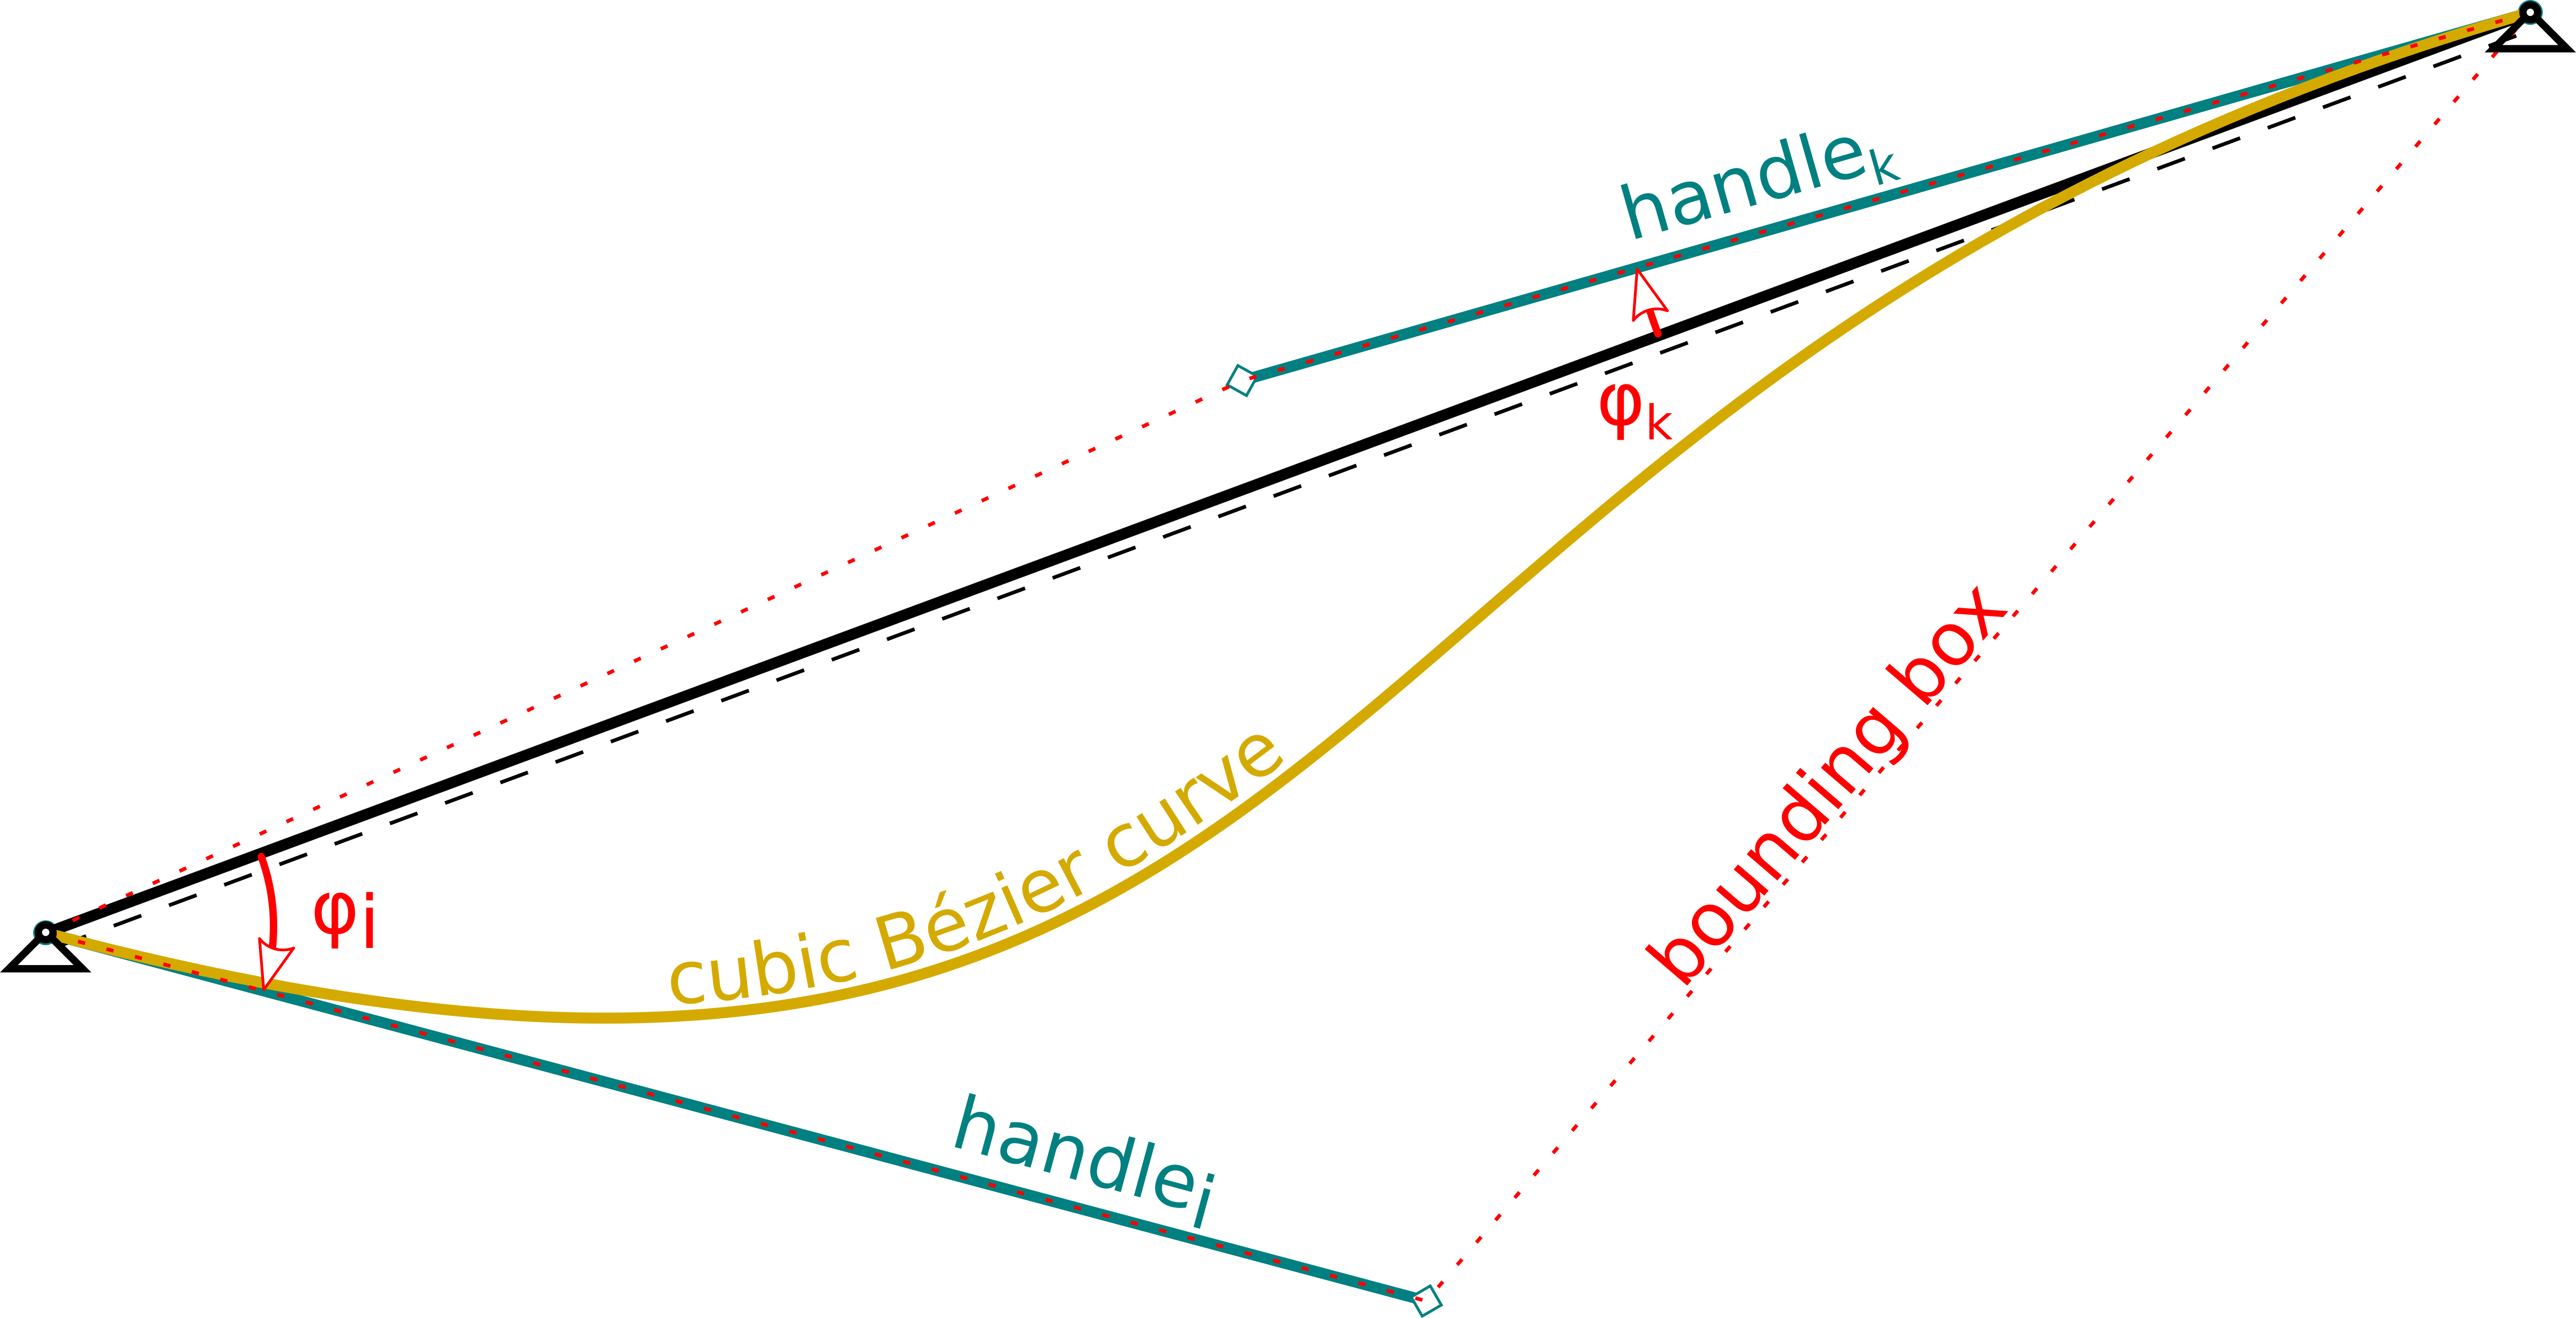
\includegraphics[width=0.9\textwidth]{cube_bezier.png}%
    \caption{Cubic B\'{e}zier curve}%
    \label{fig:cubeBezier}%
\end{figure}

The displacement and rotation at points $P_0$ and $P_3$ is known from the displacement vector $d$. Therefor the points are placed at:

\begin{equation*} \label{bezierHandles}
\begin{aligned}
P_0(x) &= node_n(x) + d_n^x \\
P_0(y) &= node_n(y) + d_n^y \\
P_3(x) &= node_{n+1}(x) + d_{n+1}^x \\
P_3(y) &= node_{n+1}(y) + d_{n+1}^y \\
\varphi_i &= d_n^r \\
\varphi_k &= d_{n+1}^r
\end{aligned}
\end{equation*}

In a first approximation the handle length ($\lvert\overrightarrow{P_0P_1}\lvert , \lvert\overrightarrow{P_3P_2}\lvert$) is set to one half of the strut length. This already turns out to produce qualitatively good results.
To increase accuracy even further, a relationship between handle length, stiffness and load could be developed but is not persued in this thesis. 

\section{Sparse Matrix Data Type}
\label{sec:sparsematrix}

In this thesis the \textit{scipy} (\cref{sec:depend}) datatype \textit{ndarray} was used to store the matrices. This tracks all indices but the matrices are symmetric and even the global stiffness matrix $K_G$ (\cref{fullstiffnessmatrix}) only contains non-zero values three columns and rows above and below the diagonal.
A sparse matrix datatype like \textit{CSR} (Compressed Sparse Row Format) or \textit{COO} (Coordinate list) could be used to optimize for memory usage.
Or even a custom datatype that tracks only the indices containing non-zero values above the diagonal.




\appendix
%\chapter{Appendix}
\cleardoublepage
\phantomsection
\addcontentsline{toc}{chapter}{\listfigurename}
\listoffigures

\cleardoublepage
\phantomsection
\addcontentsline{toc}{chapter}{Bibliography}
\printbibliography

\cleardoublepage
\phantomsection
\addcontentsline{toc}{chapter}{Resources}

\chapter*{Resources}

\textit{Github Repository} [\url{https://github.com/couchsofa/structana}]\linebreak
The program is under continued developement. The code base can be found at the above link on Github.

\cleardoublepage
\phantomsection
\addcontentsline{toc}{chapter}{Declaration}

\chapter*{Declaration}

I hereby declare, that I am the sole author and this thesis has been composed by me and is based on my own work, unless
stated otherwise. No other sources or learning aids, other than those listed, have been used. Furthermore, I declare that I have acknowledged the work of others by providing detailed references of said work.
All references and verbatim extracts have been quoted, and all sources of information, including graphs and data sets, have been specifically acknowledged. 

\vspace*{\fill}

\begin{tabular}{@{}p{.5in}p{4in}@{}}
& \hrulefill \\
& \GetAuthor \\
& \date{\today{}, Karlsruhe}\\
\end{tabular}

\vspace*{\fill}




\end{document}